\section{Figures}
\label{figures}

\begin{figure}[h]
	\centering
    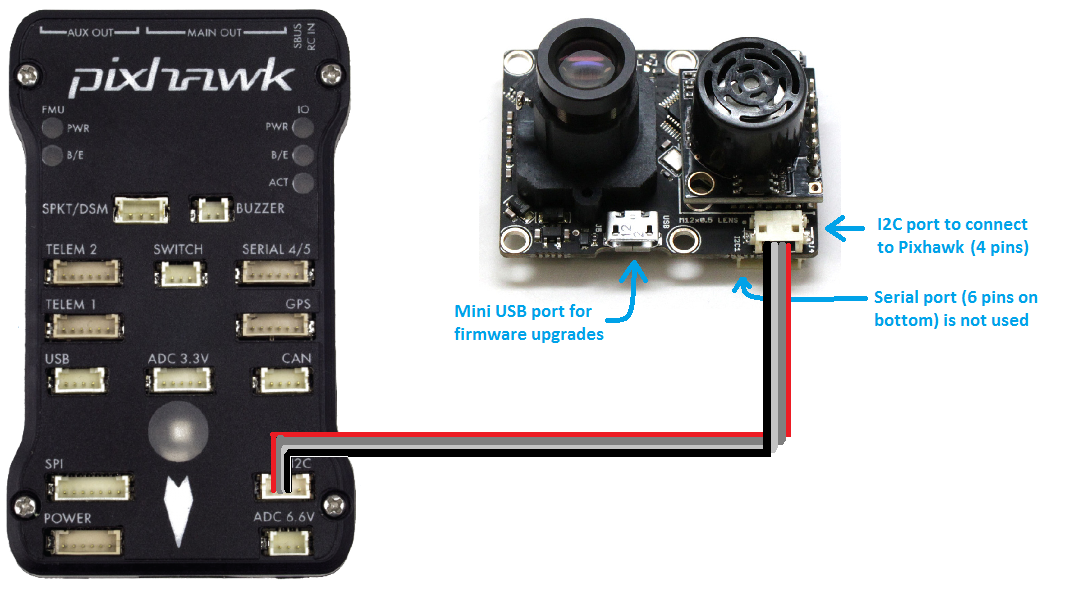
\includegraphics[width=300px]{graphics/PixhawkPX4Flow.png}
	\caption{Pixhawk PX4 Flow Connection}
	\label{fig:pixhawk_px4_flow_connection}
\end{figure}

\begin{figure}[h]
	\begin{lstlisting}[basicstyle=\scriptsize]
class OpticalFlow { //...
public: //...
	bool enabled() const { return _enabled; }
	bool healthy() const { return backend != NULL && _flags.healthy; }
	uint8_t quality() const { return _state.surface_quality; }
	const Vector2f& flowRate() const { return _state.flowRate; }
	const Vector2f& bodyRate() const { return _state.bodyRate; }
	uint8_t device_id() const { return _state.device_id; }
    //...
    struct OpticalFlow_state {
    	uint8_t device_id;
    	uint8_t  surface_quality;
    	Vector2f flowRate;
    	Vector2f bodyRate;
    };
private: //...
};
	\end{lstlisting}
	\caption{Optical Flow Sensor \ac{API}}
	\label{fig:optical_flow_api}
\end{figure}

\begin{figure}[h]
	\begin{lstlisting}[basicstyle=\scriptsize]
class RangeFinder {
public: //...
	enum RangeFinder_Status {
		RangeFinder_NotConnected = 0,
		RangeFinder_NoData,
		RangeFinder_OutOfRangeLow,
		RangeFinder_OutOfRangeHigh,
		RangeFinder_Good
	};
	
	struct RangeFinder_State {
		uint8_t instance;
		uint16_t distance_cm;
		uint16_t voltage_mv;
		enum RangeFinder_Status status;
		uint8_t range_valid_count;
		bool pre_arm_check;
		uint16_t pre_arm_distance_min;
		uint16_t pre_arm_distance_max;
	};
	//...
	uint16_t distance_cm() const { return distance_cm(primary_instance); }
	uint16_t voltage_mv() const { return voltage_mv(primary_instance); }
	int16_t ground_clearance_cm() const { return _ground_clearance_cm[primary_instance]; }
	RangeFinder_Status status(void) const { return status(primary_instance);
	//...
private: //...
};
	\end{lstlisting}
	\caption{Range Finder \ac{API}}
	\label{fig:range_finder_api}
\end{figure}

\begin{figure}[h]
	\centering
    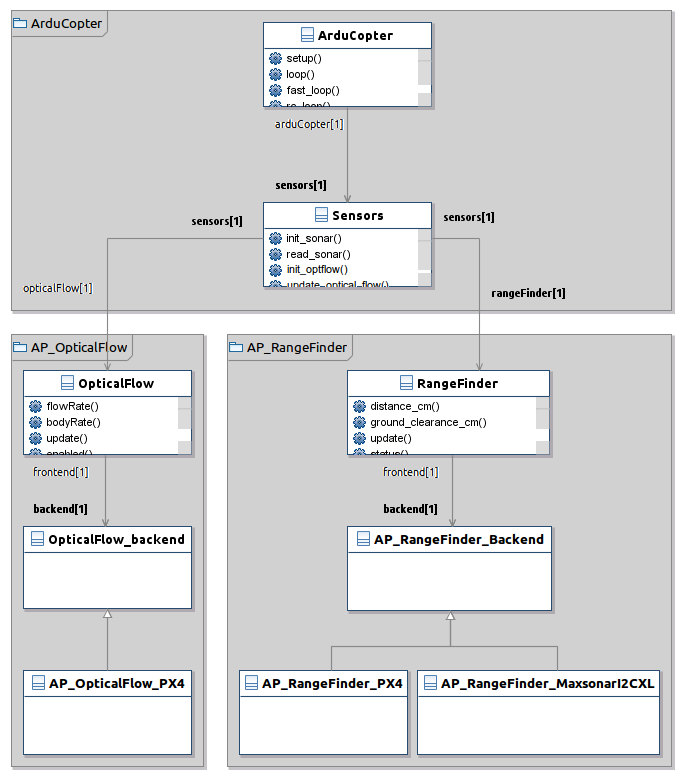
\includegraphics[width=400px]{graphics/OpticalFlowDiagram.png}
	\caption{PX4 Optical Flow Sensor Board \ac{API}}
	\label{fig:of_sensor_board_api}
\end{figure}

\begin{figure}[h]
	\begin{lstlisting}[basicstyle=\scriptsize]
static void stabilize_run()
{
    //...
    // in the stabilizing flight mode check the current flight envelope
    // measured by the optical flow sensor
    checkEnvelope();
    //...
}

#define BODY_RATE_ENVELOPE 4.0f
#define FLOW_RATE_ENVELOPE 1.0f
#define MAX_ALT 1.0f

static bool checkBodyRateEnvelope() {
        Vector2f bodyRate = optflow.bodyRate();
        return ((bodyRate.x > -BODY_RATE_ENVELOPE) && (bodyRate.y < BODY_RATE_ENVELOPE));
}

static bool checkFlowRateEnvelope() {
        Vector2f flowRate = optflow.flowRate();
        return ((flowRate.x > -FLOW_RATE_ENVELOPE) && (flowRate.y < FLOW_RATE_ENVELOPE));
}

static bool checkAltitudeEnvelope() {
        float hagl = 0.0f;
        ahrs.get_NavEKF().getHAGL(hagl);
        return (hagl <= MAX_ALT);
}

static void checkEnvelope() {
        // if the flight envelope is violated, then notify an envelope alert
        // notification subscribers include the tone alert and LED
        if (!checkBodyRateEnvelope() || !checkFlowRateEnvelope() || !checkAltitudeEnvelope()) {
                hal.console->printf("envelope violated\n");
                AP_Notify::flags.envelope_alert = true;
        } else {
                hal.console->printf("envelope satisfied\n");
                AP_Notify::flags.envelope_alert = false;
        }
}
	\end{lstlisting}
	\caption{Application Snippets}
	\label{fig:application_snippets}
\end{figure}

\clearpage
\section{Acronyms}
\label{acronyms}

\begin{acronym}
	\acro{AHRS}{Attitude and Heading Reference System}\\
		An attitude and heading reference system consists of sensors on
		three axes that provide attitude information for aircraft, including
		heading, pitch and yaw.They are designed to replace traditional
		mechanical gyroscopic flight instruments and provide superior
		reliability and accuracy.
		\footnote{http://en.wikipedia.org/wiki/Attitude\_and\_heading\_reference\_system}
	\acro{API}{Application Programming Interface}\\
		In computer programming, an application programming interface is a set
		of routines, protocols, and tools for building software applications.
		An API expresses a software component in terms of its operations,
		inputs, outputs, and underlying types. An API defines functionalities
		that are independent of their respective implementations, which allows
		definitions and implementations to vary without compromising each
		other.
		\footnote{http://en.wikipedia.org/wiki/Application\_programming\_interface}
	\acro{CPS}{Cyber-Physical System}\\
		A cyber-physical system is a system of collaborating computational
		elements controlling physical entities. Today, a precursor generation
		of cyber-physical systems can be found in areas as diverse as
		aerospace, automotive, chemical processes, civil infrastructure,
		energy, healthcare, manufacturing, transportation, entertainment, and
		consumer appliances.
		\footnote{http://en.wikipedia.org/wiki/Cyber-physical\_system}
	\acro{HAL}{Hardware Abstraction Layer}\\
		Hardware abstractions are sets of routines in software that emulate
		some platform-specific details, giving programs direct access to the
		hardware resources.
		\footnote{http://en.wikipedia.org/wiki/Hardware\_abstraction}
	\acro{II}{Industrial Internet}\\
		The Industrial Internet refers to the integration of complex physical
		machinery with networked sensors and software.
		\footnote{http://en.wikipedia.org/wiki/Industrial\_Internet}
	\acro{IIoT}{Industrial Internet of Things}\\
		The Industrial Internet of Things is a subdiscipline of the \acs{IoT},
		which describes IP-enabled systems in factories, offices and other
		commercial (and sometimes government) facilities. It is the part of the
		\acs{IoT} that focuses on how smart machines, networked sensors and
		sensor analytics can help improve business-to-business initiatives
		across a wide variety of industries, especially manufacturing.
		\footnote{http://itlaw.wikia.com/wiki/Industrial\_Internet\_of\_Things}
	\acro{IoT}{Internet of Things}\\
		The Internet of Things is the network of physical objects or "things"
		embedded with electronics, software, sensors and connectivity to enable
		it to achieve greater value and service by exchanging data with the
		manufacturer, operator and/or other connected devices.
		\footnote{http://en.wikipedia.org/wiki/Internet\_of\_Things}
	\acro{LED}{Light-Emitting Diode}
		A light-emitting diode is a two-lead semiconductor light source. It is
		a pn-junction diode, which emits light when activated. When a suitable
		voltage is applied to the leads, electrons are able to recombine with
		electron holes within the device, releasing energy in the form of
		photons.
		\footnote{http://en.wikipedia.org/wiki/Light-emitting\_diode}
	\acro{SoSs}{System of Systems}\\
		System of systems is a collection of task-oriented or dedicated systems
		that pool their resources and capabilities together to create a new,
		more complex system which offers more functionality and performance
		than simply the sum of the constituent systems.
		\footnote{http://en.wikipedia.org/wiki/System\_of\_systems}
	\acro{ToE}{Theory of Everything}\\
		A theory of everything or final theory, ultimate theory, or master
		theory is a hypothetical single, all-encompassing, coherent theoretical
		framework of physics that fully explains and links together all
		physical aspects of the universe.
		\footnote{http://en.wikipedia.org/wiki/Theory\_of\_everything}
	\acro{UAV}{Unmanned Aerial Vehicle}\\
		An unmanned aerial vehicle, known in the mainstream as a drone and also
		referred to as an unpiloted aerial vehicle and a remotely piloted
		aircraft by the International Civil Aviation Organization, is an
		aircraft without a human pilot aboard.
		\footnote{http://en.wikipedia.org/wiki/Unmanned\_aerial\_vehicle}
	\acro{ULSS}{Ulta-Large-Scale System}\\
		Ultra-large-scale system is a term used in fields including Computer
		Science, Software Engineering and Systems Engineering to refer to
		software intensive systems with unprecedented amounts of hardware,
		lines of source code, numbers of users, and volumes of data.
		\footnote{http://en.wikipedia.org/wiki/Ultra-large-scale\_systems}
\end{acronym}